\documentclass{sigchi}

% Remove or comment out these two lines for final version
\toappear{ Permission to make digital or hard copies of all or part of
  this work for personal or classroom use is granted without fee
  provided that copies are not made or distributed for profit or
  commercial advantage and that copies bear this notice and the full
  citation on the first page. To copy otherwise, or republish, to post
  on servers or to redistribute to lists, requires prior specific
  permission and/or a fee.

Gamification'13, October 2-4, 2013, Stratford, ON, Canada.

Copyright 2013 ACM 978-1-XXXX-XXXX-X/XX/XX...\$10.00.
}

\pagenumbering{arabic}% Arabic page numbers for submission. 

% Use \toappear{...} to override the default ACM copyright statement (e.g. for preprints).

% Load basic packages
\usepackage{balance}  % to better equalize the last page
\usepackage{graphicx} % for EPS, load graphicx instead
\usepackage{times}    % comment if you want LaTeX's default font
\usepackage{url}      % llt: nicely formatted URLs
\usepackage{paralist} % compact lists


\usepackage{subfigure}
\graphicspath{{figures/}}

% llt: Define a global style for URLs, rather that the default one
\makeatletter
\def\url@leostyle{%
  \@ifundefined{selectfont}{\def\UrlFont{\sf}}{\def\UrlFont{\small\bf\ttfamily}}}
\makeatother
\urlstyle{leo}

% To make various LaTeX processors do the right thing with page size.
\def\pprw{8.5in}
\def\pprh{11in}
\special{papersize=\pprw,\pprh}
\setlength{\paperwidth}{\pprw}
\setlength{\paperheight}{\pprh}
\setlength{\pdfpagewidth}{\pprw}
\setlength{\pdfpageheight}{\pprh}

%% Puts space after macros, unless followed by punctuation
\usepackage{xspace}

%%% Personal macros
%% Tired of typing CO2 so many times, requires xspace package
\newcommand{\COtwo}{CO\ensuremath{_2}\xspace}
%% Hawai`i with okina
\newcommand{\Hawaii}{Hawai`i\xspace}
%% Hawai`ian with okina
\newcommand{\Hawaiian}{Hawai`ian\xspace}
%% Manoa with kahako
\newcommand{\Manoa}{M\=anoa\xspace}

% Make sure hyperref comes last of your loaded packages, 
% to give it a fighting chance of not being over-written, 
% since its job is to redefine many LaTeX commands.
\usepackage[dvips]{hyperref}
\hypersetup{
pdftitle={Serious Game Framework Evaluation: A Case Study of Makahiki},
pdfauthor={LaTeX},
pdfkeywords={SIGCHI, proceedings, archival format},
bookmarksnumbered,
pdfstartview={FitH},
colorlinks,
citecolor=black,
filecolor=black,
linkcolor=black,
urlcolor=black,
breaklinks=true,
}

%% Make links to captions point to the figure, not just the caption at bottom
\usepackage[all]{hypcap}

% create a shortcut to typeset table headings
\newcommand\tabhead[1]{\small\textbf{#1}}

%% Since I'm using the LaTeX Makefile that uses dvips, I need this
%% package to make URLs break nicely
\usepackage{breakurl}

% End of preamble. Here it comes the document.
\begin{document}

\title{SGSEEM: Evaluating Serious Game Frameworks\\ from a Stakeholder Experience Perspective}

% Note that submissions are blind, so author information should be omitted
%\numberofauthors{5}
%\author{
%  \alignauthor Yongwen Xu, Philip M. Johnson, Carleton A. Moore, Robert S. Brewer, Jordan Takayama\\
%    \affaddr{Department of Information and Computer Sciences}\\
%    \affaddr{University of Hawaii at Manoa}\\
%    \affaddr{Honolulu, HI, USA}\\
%    \email{\{yxu, johnson, cmoore, rbrewer, jktakaya\}@hawaii.edu}\\
%}

\maketitle

\begin{abstract}
% 150 words max
  Evaluation of serious game frameworks is emerging as an important area of research. 
  This paper describes an evaluation mechanism called the
  Serious Game Stakeholder Experience Evaluation Method (SGSEEM). SGSEEM is designed to
  provide detailed insights into the strengths and weaknesses of serious game frameworks
  through a stakeholder perspective based approach.

  In this paper, we report on the use of SGSEEM to evaluate
  Makahiki, an open source serious game framework for sustainability.  Makahiki 
  facilitates the development of serious games for the purpose of education and
  behavioral change regarding energy and water consumption. Our results provide useful
  insights into both Makahiki as a serious game framework and SGEEM as an evaluation method.
\end{abstract}

\keywords{
	serious games; framework evaluation; sustainability
}

\category {H.5.m.} {Information Interfaces and Presentation (e.g., HCI)} {Miscellaneous} {K.8.0.} {Personal Computing} {Games}

%\\
%\textcolor{red}{See: \url{http://www.acm.org/about/class/1998/}
%for more information and the full list of ACM classifiers and descriptors. 
%Mandatory section: On the submission page
%only the classifiers' letter-number combination will need to be entered.}


\terms{
	Serious Game; Evaluation; Game Design; Case study.
}

\section{Introduction}

Serious games (games with additional goals beyond just entertainment) have been a topic
of academic research for decades~\cite{Zyda2005}. Such games show great potential as
interactive media that provide engaging interfaces in various serious
contexts~\cite{mcgonigal2011reality,reeves2009total}. The recent phenomenon of
gamification~\cite{Deterding2011mt} also calls for game-related research in areas beyond
traditional entertainment purposes.

One fundamental question in assessing a serious game is the extent to which the
game achieves its ``serious'' purpose.  This is quite different from 
traditional entertainment games, in which assessment focuses on usability or
playability~\cite{song2007new}. In the field of serious games, there is an increasing
focus on the methodology of research and evaluation~\cite{Mayer2012233}. De Freitas and
Oliver describe a four dimensional framework~\cite{de2006can} for evaluating an
educational game, consisting of: the context, the pedagogy, the representation, and the
learner (or player). Harteveld proposes an alternative approach called ``Triadic Game
Evaluation''~\cite{harteveld2010triadic}, consisting of three perspectives: Reality,
Meaning, and Play.

The above approaches focus on evaluation of a single game, as opposed to a game {\em
  framework}. Game frameworks (also known as game engines) are ``comprised of a collection
of different tools, utilities, and interfaces that hide the low-level details of the
various tasks that make up a game''~\cite{sherrod2006ultimate}. One of the benefits of
using a serious game framework is that, if correctly designed, it will provide useful and
reusable ``building blocks'' with which to develop a variety of serious games.  These
building blocks enable the serious game developer to focus more time and thought on
content and results instead of on infrastructure.  Yet how are we to know if a serious
game framework has been ``correctly designed''?

To help answer this question, this paper proposes a method for evaluating serious game
frameworks, called the Serious Game Stakeholder Experience Evaluation Method (SGSEEM). In
a nutshell, SGSEEM identifies the most important stakeholders of a serious game framework
and provides a method for gaining insight into whether the framework is effective and
efficient with respect to each stakeholders' needs.

To understand SGSEEM, we will start by briefly introducing Makahiki, our serious game
framework for sustainability, and how its development motivated us to create the SGSEEM
method. We then describe our preliminary results from the application of SGSEEM to
Makahiki. We conclude with the insights this evaluation process provides for our own work
on Makahiki as well as for serious game design in general.


\section{Motivation for SGSEEM}

Sustainability education and conservation have become an international
imperative due to the rising cost of energy, increasing scarcity of
natural resources, and irresponsible environmental practices. Over the
past decade, energy and water challenges have become focal
points for sustainability efforts at both university and industry
campuses. For example, college residence hall energy competitions have
been a widespread mechanism for engaging students in energy issues,
with more than 160 taking place or being planned for the 2010--2011
academic year in North America~\cite{Hodge2010}.

Designers of such challenges typically have three choices for
information technology support: (a) build their own custom in-house
solution (as was done at Oberlin College in
2006~\cite{petersen-dorm-energy-reduction}); (b) out-source to a
commercial provider (as was done at the University of British Columbia
in 2011); or (c) use a minimal tech solution such as a web page and
manual posting of data and results (as was done at Harvard in 2012).

None of these choices are ideal: the custom in-house solution requires
sophisticated design and implementation skills; out-sourcing can be
financially expensive and impedes evolution; and the minimal tech
solution does not fully leverage the possibilities of advanced
information technology.

To provide a new alternative to these three choices, we designed and implemented
an open source serious game framework for sustainability called
Makahiki~\cite{csdl2-12-06}.  Makahiki is an extensible software system with a variety
of common services for developing sustainability games including: authentication; game
mechanics such as leaderboards, points, and badges; a variety of built-in games and
content focused on sustainability; a responsive user interface; cloud-based deployment;
and the ability to customize the game to the needs of individual organizations.  
Figure \ref{fig:Makahiki-Home-Page} illustrates a home page implemented using Makahiki.

\begin{figure}[ht!]
  \center
  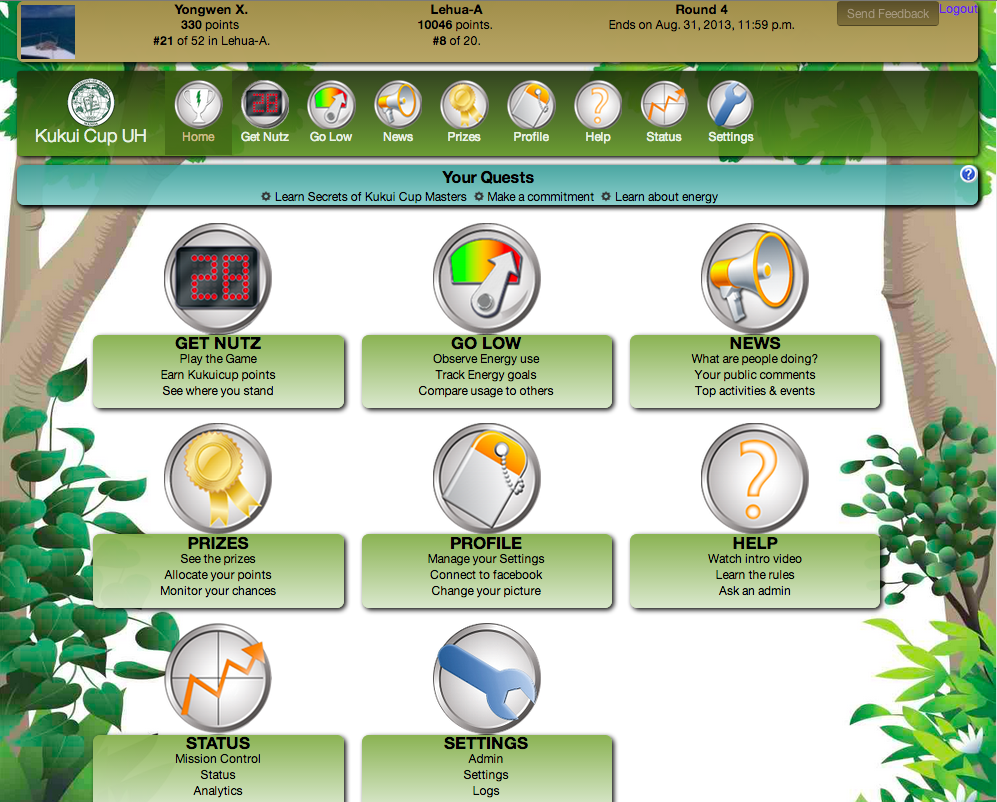
\includegraphics[width=\columnwidth]{kukuicup-home}
  \caption{Makahiki Game Instance}
  \label{fig:Makahiki-Home-Page}
\end{figure}

To explore the ability of the Makahiki framework to support sustainability games in
different environments, we ran challenges at three different organizations in Fall 2012:
The University of Hawaii, Hawaii Pacific University, and the East-West Center. While these
experiences provided anecdotal evidence that Makahiki constitutes a framework, we realized
that a more rigorous evaluation would yield better insight into its current quality and
requirements for future enhancement.

Upon review of the literature, we found little prior work concerning formal evaluation for
the particular needs of serious game frameworks. As a result, we designed SGSEEM, and
began applying it to gain better insight into Makahiki and serious game evaluation in general.

\section{Serious Game Stakeholder Experience Evaluation Method (SGSEEM)}

The goal of SGSEEM is to determine to what extent the serious game
framework under evaluation, as an Information Technology (IT)
infrastructure, can effectively and efficiently support the
development and play of a serious game.

An \emph{effective} serious game framework can produce a game with the desired outcome
with respect to its ``serious'' goals for the players. For example, an effective serious
game framework for energy education and conservation produces a game that increases
players' energy literacy and reduces their energy consumption during (and, hopefully,
after) the game. Because the goals of serious games are always subject specific, the
desired effect of a serious game for sustainability is, for example, different than the desired effect
of a serious game for language learning.  In this paper, we will 
refer to subject-specific goals relevant to sustainability, but users of SGSEEM in other
domains will substitute goals for their area. 

An \emph{efficient} serious game framework can support the
full life cycle of game development, execution, and wrap-up of the
serious game, including design, management, administration, development,
and improvement of the game.

\subsection{Methodology}

Creswell \cite{creswell2003} categorizes research methods into three approaches:
quantitative, qualitative, and mixed-methods, according to what constitutes knowledge and
how knowledge is best acquired. SGSEEM is a mixed-methods approach with both qualitative
and quantitative data collection and analysis.

In SGSEEM, qualitative analysis involves structured interviews and questionnaires 
designed to gain insight about stakeholder experiences with the framework under
study. In addition to qualitative analysis, SGSEEM also employs quantitative analysis involving
the analytical data recorded by the system, including website logs, player interaction
logs, feedback, resource usage, etc.

\subsection{Stakeholders}

There are a great variety of potential stakeholders in serious games.
The following are the stakeholders we identified for Makahiki:

\begin{compactitem}
\item \emph{Players}: those who participate in the game play.
\item \emph{System Admins}: those who install and maintain the technological game infrastructure.
\item \emph{Game Designers}: those who design the content and game mechanics.
 \item \emph{Game Managers}: those who manage the game during the period of game play.
\item \emph{Developers}: those who extend, enhance and debug the game framework.
\item \emph{Researchers}: those who are conducting research using the game framework.
\item \emph{Spectators}: those who do not participate in the game
  play but are interested in the game and the results of game play.
\item \emph{Community partners}: those who partner
  with the game organizers to help run the game (such as coordinating real-world events as part of the game).
\item \emph{Facilities}: those who are responsible for the resources (energy, water, etc)
  associated with the game.
\item \emph{Funding organizations}: the organizations who provide
  funding to the project.
\end{compactitem}

The overall success of a serious game framework for sustainability depends on the
individual success of all of these stakeholders. However, as SGSEEM focuses on the software
infrastructure, it does not address the spectator, community partner, facilities, and funding
organization stakeholders. These are important stakeholders but outside the scope of our
evaluation method.

Our case study evaluation of Makahiki using SGSEEM evaluates: (1) aspects of 
effectiveness of the system for Players, and (2) aspects of
efficiency for System Admins, Game Designers, Game Managers, Developers, and Researchers.

\autoref{fig:evaluation-framework} provides an overview of the evaluation framework. The
following sections describe in detail the evaluation mechanism for each stakeholder.

\begin{figure}[ht!]
  \centering
  \begin{tabular}{|c|c|}
    \hline
    \multicolumn{1}{|p{0.3\columnwidth}|}{\centering\tabhead{Stakeholder}} &
    \multicolumn{1}{|p{0.6\columnwidth}|}{\centering\tabhead{Evaluation Goal}} \\
    \hline
    \multicolumn{1}{|p{0.3\columnwidth}|}{Players} &
    \multicolumn{1}{|p{0.6\columnwidth}|}{Effectiveness of the game
      to players in terms of literacy and behavior change in
      sustainability, player engagement} \\ 
    \hline
    \multicolumn{1}{|p{0.3\columnwidth}|}{System admins} &
    \multicolumn{1}{|p{0.6\columnwidth}|}{Efficiency in administrating the system} \\
    \hline
    \multicolumn{1}{|p{0.3\columnwidth}|}{Game designers} &
    \multicolumn{1}{|p{0.6\columnwidth}|}{Efficiency in designing a game} \\
    \hline
    \multicolumn{1}{|p{0.3\columnwidth}|}{Game managers} &
    \multicolumn{1}{|p{0.6\columnwidth}|}{Efficiency in managing a game} \\
    \hline
    \multicolumn{1}{|p{0.3\columnwidth}|}{Developers} &
    \multicolumn{1}{|p{0.6\columnwidth}|}{Efficiency in developing a game or enhancing the system} \\
    \hline
    \multicolumn{1}{|p{0.3\columnwidth}|}{Researchers} &
    \multicolumn{1}{|p{0.6\columnwidth}|}{Efficiency in performing research} \\
    \hline
  \end{tabular}
  \caption{Overview of SGSEEM}
  \label{fig:evaluation-framework}
\end{figure}

\subsubsection{1. Player Effectiveness}

SGSEEM assesses the ``effectiveness'' of a serious game framework for the
Player stakeholder by addressing three questions: (a) To what extent does the game
increase player's literacy in sustainability? (b) To what extent does
the game produce positive player behavior change in sustainability?
(c) To what extent does the game engage players?

\autoref{fig:pre-post-eval} illustrates the process for player
effectiveness evaluation, which involves a pre-game and post-game
measurement for literacy and behavior change, as well as the in-game
data logging to measure the level of player engagement.

\begin{figure}[ht!]
  \center
  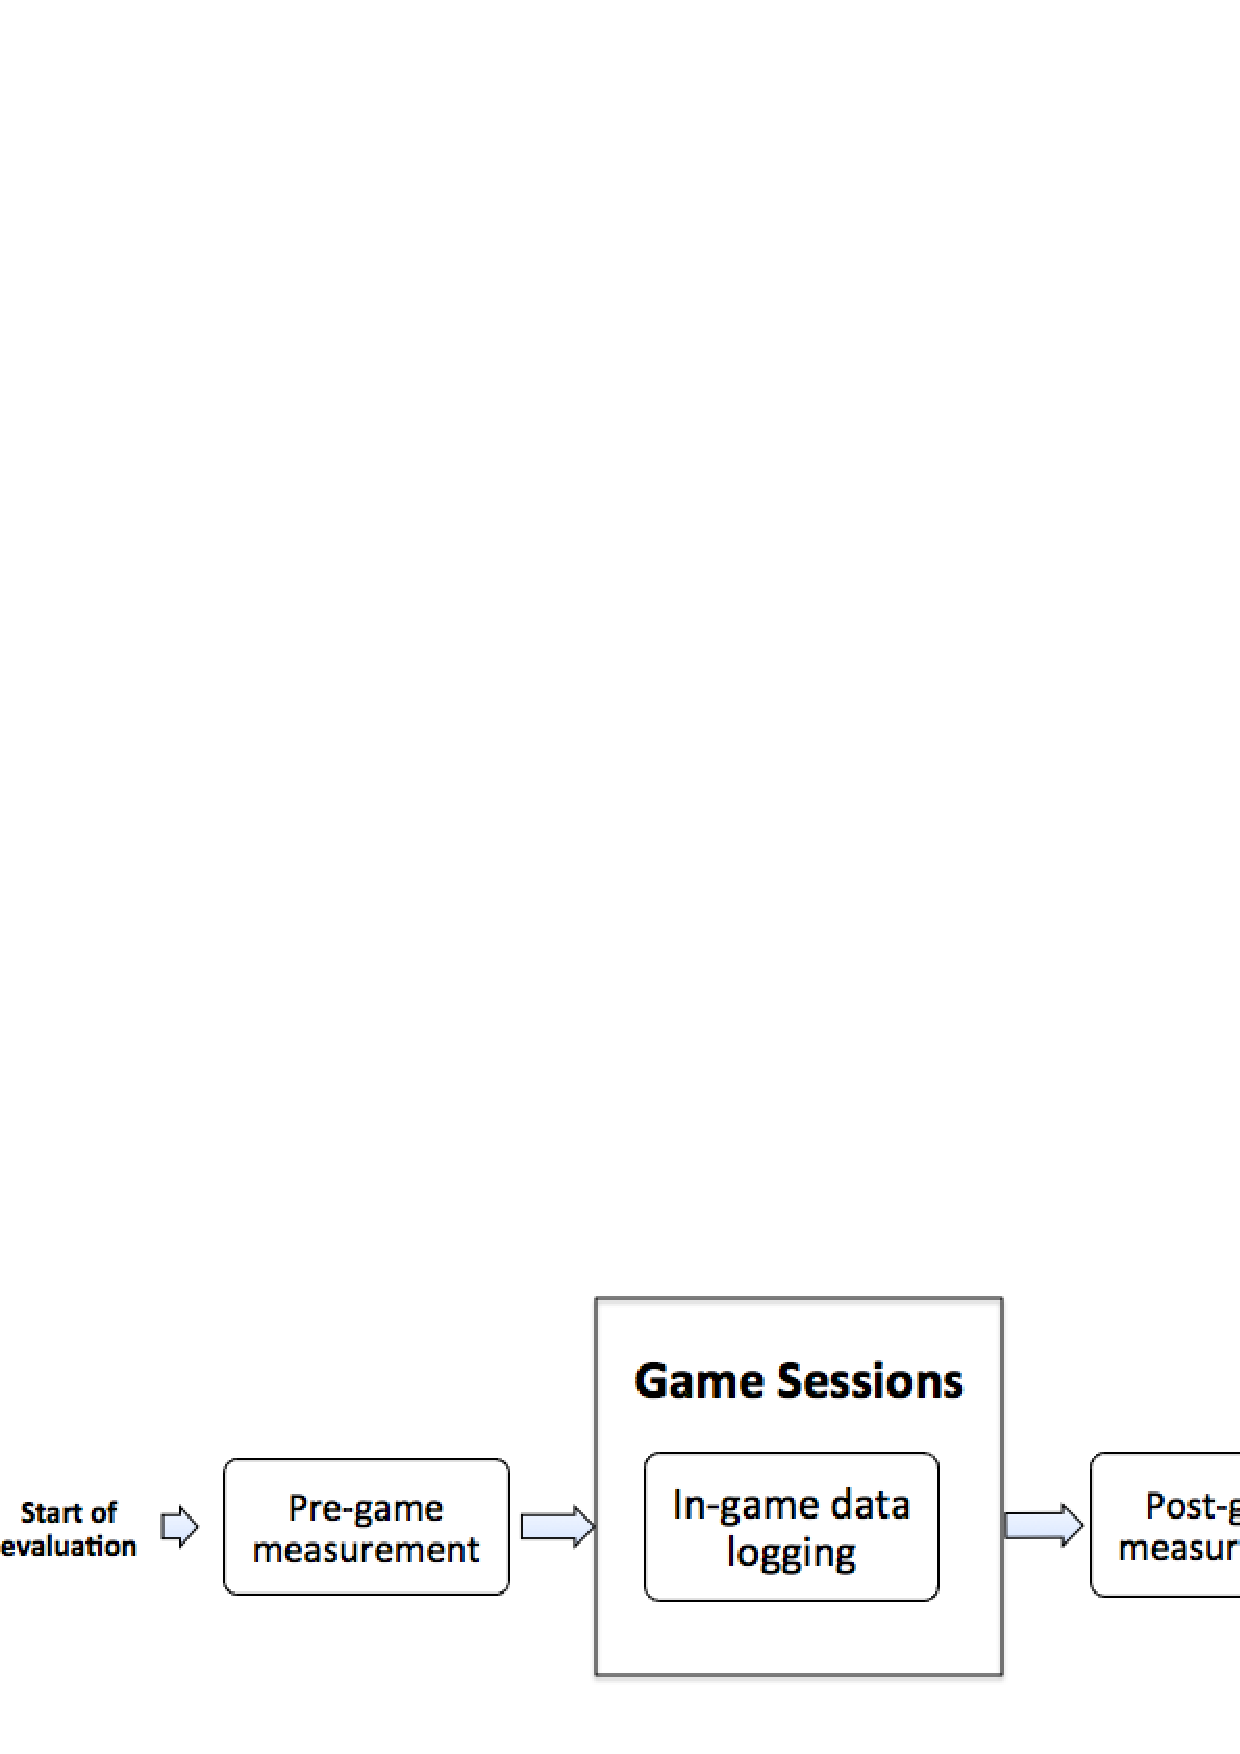
\includegraphics[width=\columnwidth]{pre-post-eval}
  \caption{Player Effectiveness Evaluation Process}
  \label{fig:pre-post-eval}
\end{figure}

\emph {(a) Literacy assessment:} One important goal of a serious
game for sustainability is to produce a change in knowledge in the
players. A literacy assessment can indicate whether this goal is being met.

SGSEEM uses an approach similar to that described in \cite{csdl2-10-08} to
assess the impact of the game on player literacy. In general, a set of literacy survey
questionnaires are presented to a random selection of the players 
before the game. After the game ends, the same survey
(post-game) is presented to the players who responded the
pre-game survey. These two set of survey response data are
compared to understand if the game has had an impact on literacy.

The extent of players' sustainability literacy change will indicate
the degree of educational effectiveness of the serious game for
sustainability.

\emph {(b) Behavior change assessment:} Positive behavior change is
another main goal of a serious game for sustainability. A serious game
for sustainability may include some degree of resource
consumption measurement. SGSEEM uses resource consumption data before and
after the game as part of the assessment of the
players' sustainability behavior change.  A resource consumption
baseline can be established based on historical
consumption data. During and after the game, we can compare the
resource consumption with the baseline for a particular day to
understand to what extent the resource consumption has changed.

The problems with using a baseline to assess the energy reduction in the case of dormitory
energy challenges is discussed in detail by Johnson et al.~\cite{csdl2-12-08}. As a method
for evaluating the effectiveness of serious game for sustainability in a broader context
beyond the dormitory challenge, we continue to use the baseline method as one way to
assess changes in resource consumption.

In addition to resource consumption, SGSEEM can include the use of a
behavior survey to measure self-reported behavior
change. A pre-game survey is presented to the players to ask about
their current sustainability behavior, then after the game, a post-game
survey is presented to ask about the players' behavior again. These two
sets of survey response data can be compared to understand if there is
any changes.

The combination of resource consumption changes and self-reported
behavior changes can be used to assess the degree of behavior
effectiveness of the serious game for sustainability.

\emph {(c) Engagement assessment:} Player engagement is an important measure for
understanding the effectiveness of a serious game. By investigating the degree of
engagement, we can determine to what extent individuals are participating in the game, as
well as to what extent the community population is participating in the game.

Engagement has a subtle relationship to the overall effectiveness of a serious game. It is
possible for the game to be played by only a subset of the target population, but
have an impact on those not playing by virtue of their contacts with players. Gaining
better insight into this effect is an area of active study for us. 

To obtain engagement data, SGSEEM requires the framework to support the following measures
based upon system log data: 

\begin{compactitem}
\item participation rate
\item number of players per day
\item play time of a player per day
\item submissions of all player per day
\item social interaction of all player per day
\item website errors per day
\end{compactitem}

The participation rate measures the percentage of users who used the game based on the total
eligible players. In the serious game context, it indicates the level of involvement or awareness
of the serious matters. The number of players and play time per day measure how frequently the
players interact with the game. The submissions per day measures the rate of serious game
specific activities (online or real world) that players completed, while the social interaction
per day measures the rate of social interactions happened in the game between the players. At
last, the website errors per day measures the rate of errors encountered by the players while
using the game website. In general, with the opposite of website error measurement, the higher
value of these measurements are, the higher engagement level the system has.

\subsubsection{2. System Admin Efficiency}

System administrators simply install the framework and dependent libraries, do backups,
and so forth. SGSEEM assesses the efficiency of the system admin stakeholder through
interviews involving the following questions:

\begin{compactitem}
\item How much time did you require to install the system, including the dependencies?
\item How much time did you require to maintain the system?
\item What problems did you encounter?
\item Did you find it difficult to admin the system? What was difficult?
\end{compactitem}

After the interview data is acquired, the evaluator will perform qualitative data
analysis, which involves transcribing (if the interview data is in audio format),
categorizing and coding the description of reported problems or difficulties.
Once the categories of problems are coded, the evaluator will correlate the reported time
data and the coded categories to identify the area of strength (less time spent) and
weakness (problems and difficulties).

\subsubsection{3. Game Designer Efficiency}

A game designer uses the serious game framework to design and create a serious game.
A serious game framework always provides certain tools or interfaces to game designers
with the hope that these will simplify the design of a game. Such tools might involve
configuring global settings for the game, such as how long will the game run, who are the
players, and how to design individual game elements.

SGSEEM measures the efficiency of a serious game framework with respect to the Game
Designer stakeholder by addressing the following two questions: (a) How much time is
required to design an instance of a serious game using the framework? and (b) How many,
and how problematic are the errors that designers encounter during the design process?

SGSEEM requires the evaluator to first identify the sequence of tasks to be carried out by
the game designer, then acquire two sets of assessment data.
The first data set is the system log data for the interaction between the game designer
and the serious game framework. This data is used to determine how much
time it takes a designer to complete a certain design task using the game
framework, and any errors encountered. 

A second set of data is obtained by interviewing the designer and asking the following questions:
\begin{compactitem}
\item How much time did you spend to complete each design task?
\item What problems did you encounter?
\item Did you find it difficult to configure? What was difficult?
\item Did you find it difficult to design a specific game? Which one, and what was difficult?
\end{compactitem}

The interview data will be transcribed (if audio recording), categorized and coded. The time
data from the interviews will be validated by the system log data, while the descriptive problem
categories will be correlated with the system log time and error data to assess the areas of
strength and weakness of each category.

\subsubsection{4. Game Manager Efficiency}

A game manager uses the serious game framework to manage the serious game that the game
designers created. It is possible that a game manager is also the game designer.
Serious game frameworks normally provide certain interfaces for the managers to manage the
game. This may involve managing player submissions, monitoring the game state, entering
manual resource data, notifying winners of the game, etc.

SGSEEM measures the efficiency of a serious game framework with respect to the game
manager stakeholder with the following questions: (a) How much time is
required to manage an instance of a serious game using the framework? and (b) How many,
and how problematic are the errors that managers encounter during the design process?

Similar to the evaluation of game designer experience, SGSEEM requires the evaluator to
identify the tasks for managing the serious game, then
analyze two sets of data to assess game manager efficiency. The
first set of data is the system log data for the interaction between
the game manager and the serious game framework. This log data is used to
determine the time it takes a manager to complete
management tasks using the interface, and any system error he or she
encountered. 

A second set of data is obtained by interviewing the managers to answer the following
questions:

\begin{compactitem}
\item How much time did you spend to complete each managing task?
\item What problems did you encounter?
\item Did you find it difficult to manage? What was difficult?
\end{compactitem}

The analysis is similar to the game designer evaluation analysis. In the case of the same
person(s) sharing the roles of game designer and game manager, when performing interviews, the
evaluator should clarify what stakeholder role an interviewing question applies to.

\subsubsection{5. Developer Efficiency}

The developer stakeholder is different from the game designer stakeholder, in that the
game designer stakeholder tailors the framework without requiring any software
development, while the Developer stakeholder enhances, corrects, and extends the system by
manipulating code. 

To investigate how efficient it is to understand, extend, and debug a serious game
framework, SGSEEM assesses how much time it takes to develop an
enhancement to the game framework, and how many errors are encountered
during the process. This is accomplished by interviewing the developer(s) to
answer the following questions:

\begin{compactitem}
\item How much time did you spend developing and debugging an
  enhancement to the game framework?
\item What problem(s) did you encounter?
\item Did you find it difficult to understand, extend and debug the
  system? What was difficult?
\end{compactitem}

Similarly, the descriptive data will be categorized and coded. The evaluator will analyze
 the time and problem the developers reported.  The areas of strength (less time spent) and weakness (problems and difficulties) are identified from developers' perspective.

\subsubsection{6. Researcher Efficiency}

Finally, the researcher stakeholder is the one who uses the serious game framework to
investigate questions about gaming in general, human computer interaction, etc. 

To investigate how efficient it is to do research with the system, SGSEEM
assesses how much time it takes to use the system for specific research
queries, and how many errors are encountered during the process. The evaluator
interviews the researcher(s) to answer the following questions:
\begin{compactitem}
\item How much time did you spend to collect the research data for a
  specific topic?
\item What problems did you encounter when collecting the data?
\item Did you find it difficult to collect data from the system?
  What was difficult?
\end{compactitem}

\section{Case Study of Makahiki}

Now that we have described SGSEEM, this section will discuss
a case study of how we applied SGSEEM to evaluate Makahiki, our serious
game framework for sustainability. 

\subsection{Makahiki in Brief}

Makahiki is an innovative serious game framework for sustainability whose development
began in 2010. It combines both software and hardware infrastructure for the
development of sustainability challenges. Makahiki explores one section of the design
space where virtual world game mechanics are employed to affect real
world sustainability behaviors.

Makahiki consists of a configurable game framework that can be customized
to the needs of different organizations. It includes a library of
pre-built game ``widgets'' that implement a variety of game mechanics.
Using the widgets, an organization can create a custom sustainability
challenge in which players can compete individually or in teams to
earn points and reduce consumption of resources such as water or energy.
\autoref{fig:makahiki-architecture} illustrates the architecture of
Makahiki. \autoref{fig:makahiki-games} shows a few examples of the
games implemented in the Makahiki game library. More detailed
description of Makahiki can be found in ~\cite{csdl2-12-06}.

\begin{figure}[ht!]
  \center
  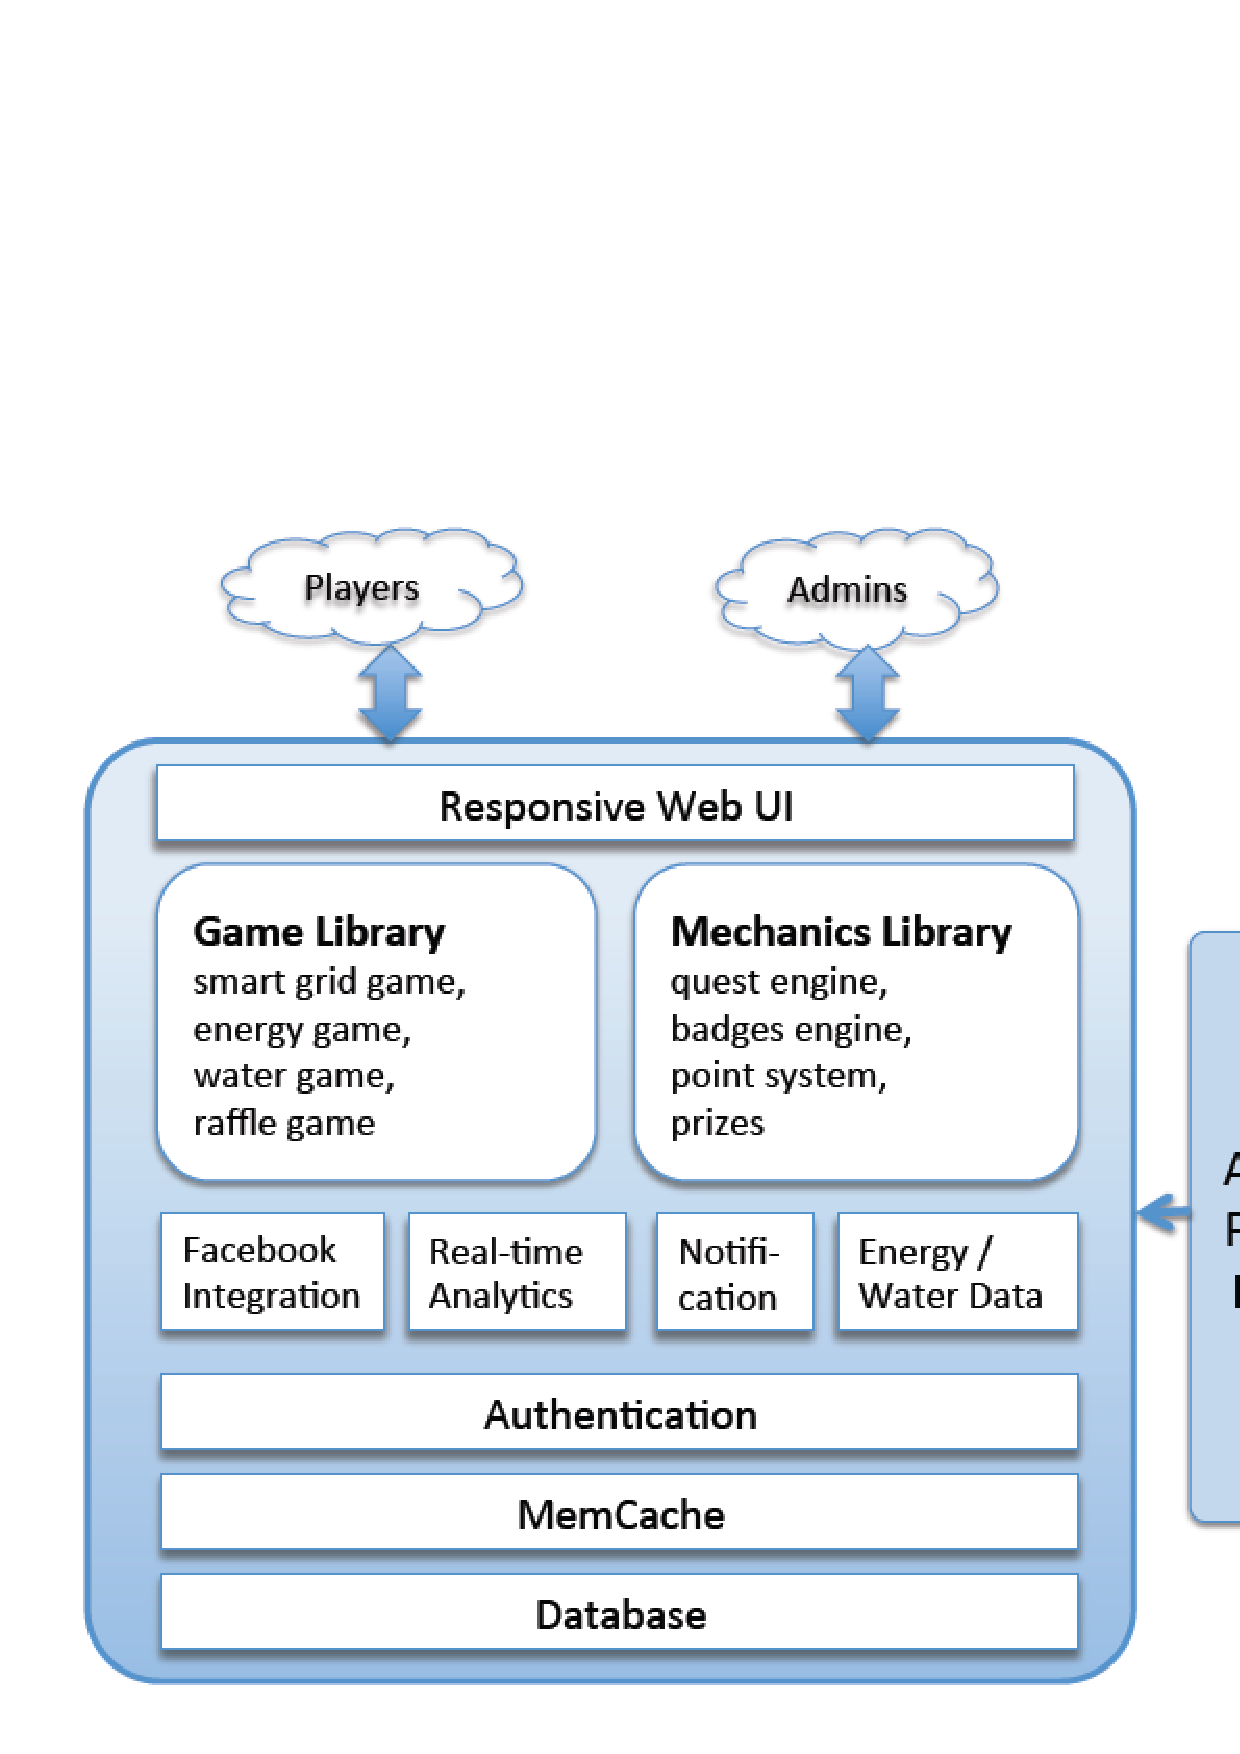
\includegraphics[width=\columnwidth]{makahiki-system-architecture}
  \caption{Architecture of Makahiki}
  \label{fig:makahiki-architecture}
\end{figure}

\begin{figure}[ht!]
	\center
		\subfigure[Smart Grid Game]{\label{fig:SmartGrid}\includegraphics[width=0.48\columnwidth]{smart-grid-game.eps}}
		\subfigure[Energy Goal Game]{\label{fig:DailyEnergyGoal}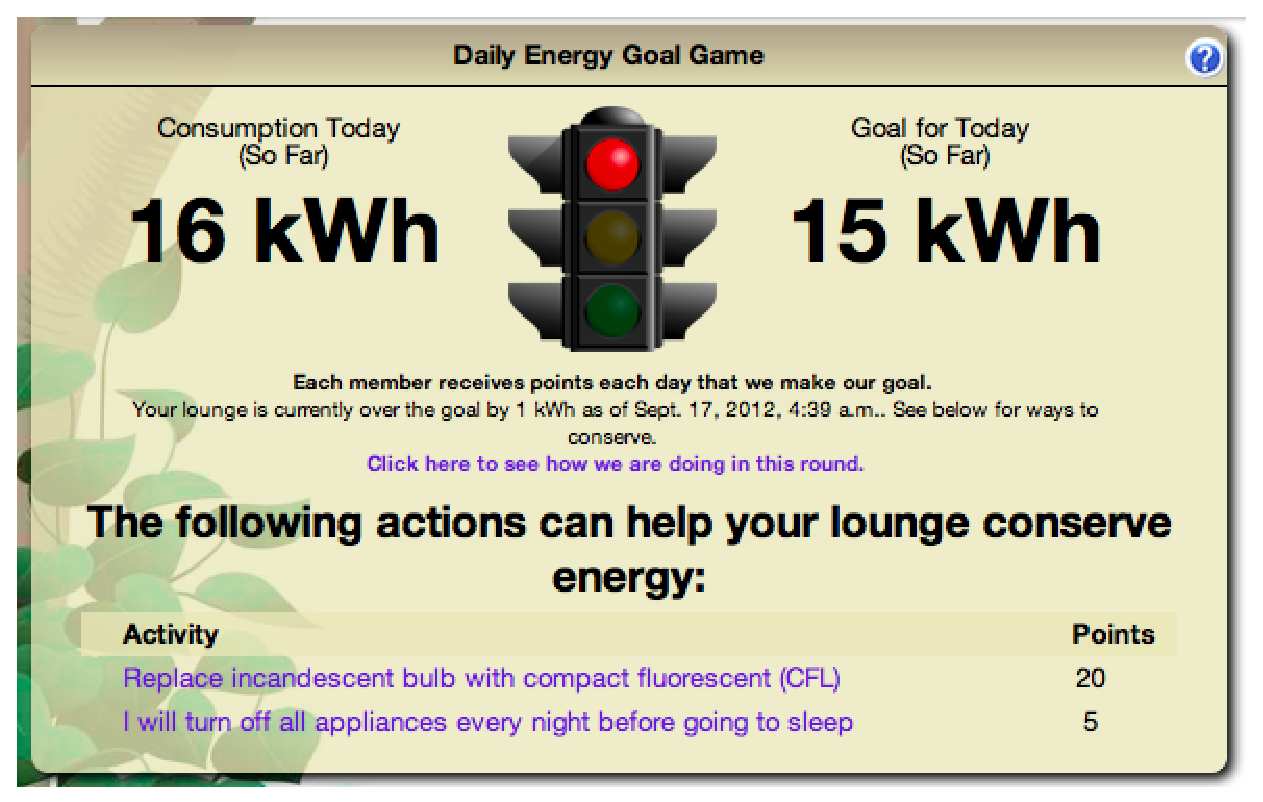
\includegraphics[width=0.48\columnwidth]{daily-energy-goal-game.eps}}
		\caption{Makahiki Game Library}
		\label{fig:makahiki-games}
\end{figure}

\subsection{Experiences with Makahiki}

We have used Makahiki to create four different Kukui Cup Energy Challenges. Kukui Cup
Energy challenges were held at the University of Hawaii (UH) in 2011 and 2012 for over
1,000 first year students living in the residence halls. Hawaii Pacific University (HPU)
held a Kukui Cup Energy challenge in Fall 2012 for about 200 students. An international
organization called the East-West Center (EWC) held a Kukui Cup Energy and Water challenge
for approximately 600 international residents living in their residence halls. Since the
halls did not have internet-enabled meters, resource consumption data had to be entered by
the game managers manually.

The successful creation of serious game challenges by three different organizations
provides evidence that Makahiki can be successfully tailored
to the needs of different organizations. First, UH and HPU used different metering
infrastructure, and EWC collected their resource data manually.  Second, while UH and HPU
challenges involved only energy consumption data, the EWC challenge involved both energy
and water consumption data. Third, the IT infrastructure at UH and HPU provided
authentication services using CAS (Central Authentication Service) and LDAP, while EWC
used the built-in Django authentication.  Fourth, the user interface was customized to
``brand'' each challenge with the logo, thematic elements, and the education contents of
the sponsoring organizations.

Besides the real world usage of Makahiki in the series of Kukui Cup challenges, we
performed in-lab evaluation experiments in 2013. Makahiki was used in a serious game
development course in Spring semester of 2013 at the Information and Computer Sciences
Department of the University of Hawaii at Manoa. There were a total of 8 students who
participated in the experiments.  The participants were either senior undergraduates or
graduate students majoring in Computer Science. During the course, the students installed
Makahiki, configured and designed a serious game instance with Makahiki, and finally
developed an enhancement to the Makahiki framework. We asked the students taking the
course to voluntarily participate in the evaluation experiments of Makahiki, using SGSEEM.

\subsection{Evaluation of Makahiki}

\subsubsection{Player Effectiveness Evaluation}

We evaluated player effectiveness regarding the 2011 Kukui Cup Challenge at the University of
Hawaii at Manoa. There were over 1000 eligible players for this challenge, who were mostly
first year college students living in the resident halls. The challenge lasted for 3
weeks.  Makahiki recorded detailed logging data from every interaction between the players
and the website.

To assess the effectiveness of the game in improving player literacy in sustainability, we
conducted two energy literacy surveys, one before the challenge (pre-game) and one after
the challenge (post-game). 24 players completed both surveys. Out of the total 19 energy
literacy questions, the average number of questions answered correctly is 7.54 before the
challenge, and 8.96 after the challenge. This result indicates an 18\% improvement on the
energy literacy.  We also surveyed non-players as a control condition, and found that
their literacy did not change, indicating that the improvement in player literacy was
indeed due to the game. 

To assess the effectiveness of the game in producing positive change in sustainability
behaviors, we recorded and analyzed energy consumption data before, during and after the
challenge.  Before the challenge, an energy usage baseline was established. During the
challenge, compared to the baseline, 12 out of the total 20 teams reduced their energy
consumption, with the highest reduction of 16.1\%. However, 3 teams actually increased
their energy consumption, with the highest increase of 11.7\%. Overall, the average
reduction of the 20 teams was very low---approximately 2\%.

To assess player engagement of the game, we calculated a variety of engagement
metrics. The results are shown in \autoref{fig:makahiki-engagement}:

\begin{figure}[ht!]
  \centering
  \begin{tabular}{|c|c|c|c}
    \hline
    \multicolumn{1}{|p{0.5\columnwidth}|}{\centering\tabhead{Measurement}} &
    \multicolumn{1}{|p{0.1\columnwidth}|}{\centering\tabhead{MIN}} &
    \multicolumn{1}{|p{0.1\columnwidth}|}{\centering\tabhead{AVG}} &
    \multicolumn{1}{|p{0.1\columnwidth}|}{\centering\tabhead{MAX}} \\
    \hline
    \multicolumn{1}{|p{0.5\columnwidth}|}{Participation rate} &
    \multicolumn{1}{|p{0.1\columnwidth}|}{13\%} &
    \multicolumn{1}{|p{0.1\columnwidth}|}{37\%} &
    \multicolumn{1}{|p{0.1\columnwidth}|}{74\%} \\
    \hline
    \multicolumn{1}{|p{0.5\columnwidth}|}{Number of players per day} &
    \multicolumn{1}{|p{0.1\columnwidth}|}{43} &
    \multicolumn{1}{|p{0.1\columnwidth}|}{85} &
    \multicolumn{1}{|p{0.1\columnwidth}|}{147} \\
    \hline
    \multicolumn{1}{|p{0.5\columnwidth}|}{Play time per day} &
    \multicolumn{1}{|p{0.1\columnwidth}|}{1 min} &
    \multicolumn{1}{|p{0.1\columnwidth}|}{27.7 mins} &
    \multicolumn{1}{|p{0.1\columnwidth}|}{8.5 hours} \\
    \hline
    \multicolumn{1}{|p{0.5\columnwidth}|}{submissions per day} &
    \multicolumn{1}{|p{0.1\columnwidth}|}{32} &
    \multicolumn{1}{|p{0.1\columnwidth}|}{266} &
    \multicolumn{1}{|p{0.1\columnwidth}|}{1110} \\
    \hline
    \multicolumn{1}{|p{0.5\columnwidth}|}{social interactions per day} &
    \multicolumn{1}{|p{0.1\columnwidth}|}{51} &
    \multicolumn{1}{|p{0.1\columnwidth}|}{208} &
    \multicolumn{1}{|p{0.1\columnwidth}|}{468} \\
    \hline
    \multicolumn{1}{|p{0.5\columnwidth}|}{website errors per day} &
    \multicolumn{1}{|p{0.1\columnwidth}|}{0} &
    \multicolumn{1}{|p{0.1\columnwidth}|}{0.6} &
    \multicolumn{1}{|p{0.1\columnwidth}|}{4} \\
    \hline
  \end{tabular}
  \caption{Makahiki Engagement Metrics}
  \label{fig:makahiki-engagement}
\end{figure}

The participation rate of this challenge is 37\%, which is very good compared to other
sustainability challenges. Over the course of the challenge, an average player spent about
27.7 minutes per day on the website. One player spent 8.5 hours on one day. There were an
average of 266 activity submissions and 208 social interactions between players per day.

In summary, SGSEEM indicates that Makahiki can be successful in achieving
player engagement and literacy improvement. SGSEEM could not provide evidence of positive change in
behavior. 


\subsubsection{System Admin Efficiency Evaluation}

System admin efficiency evaluation was determined using an in-lab experiment.  Students in
the serious game class were tasked with installing the Makahiki system into their local
computers. In order to understand how much time it takes to install Makahiki and what
problems might be encountered, we designed a Google form explaining the steps required to
install Makahiki. We asked the students to record the time they spent completing each step
and the problems they encountered. We also asked the students to provide feedback about
their installation experiences in the form of blog posts.

The Google form data shows that the average total time to successfully install Makahiki
was 1.4 hours, with a maximum time of 2 hours and the minimum time of 0.9 hour. The main
problem the students encountered during the installation was the difficulty in configuring
the Postgres database which is one of the dependent technologies of the Makahiki system.

We calculated the time for each task from the data we collected from the Google
Form, and coded the descriptive feedback reported by the students in both the Google Form and
 their blog posts. If the student reported problems in one of the tasks, we assigned the task
  a rating value of -1 (negative); if the student gave positive comments for the task, we
  assigned the task value of 1 (positive). We generalized the local installation tasks into 6
  categories which are common to a serious game framework. We aggregated all the ratings from
  the feedback of the 8 students that participated in the experiment.
  \autoref{fig:makahiki-install} shows the result of the analysis:

\begin{figure}[ht!]
  \centering
  \begin{tabular}{|c|c|c|}
    \hline
    \multicolumn{1}{|p{0.5\columnwidth}|}{\centering\tabhead{Category}} &
    \multicolumn{1}{|p{0.2\columnwidth}|}{\centering\tabhead{Average Time (minutes)}} &
    \multicolumn{1}{|p{0.15\columnwidth}|}{\centering\tabhead{Feedback rating}} \\
    \hline
    \multicolumn{1}{|p{0.5\columnwidth}|}{Setup runtime environment} &
    \multicolumn{1}{|p{0.2\columnwidth}|}{10.0} &
    \multicolumn{1}{|p{0.15\columnwidth}|}{1.4} \\
    \hline
    \multicolumn{1}{|p{0.5\columnwidth}|}{Install dependencies} &
    \multicolumn{1}{|p{0.2\columnwidth}|}{29.4} &
    \multicolumn{1}{|p{0.15\columnwidth}|}{1.3} \\
    \hline
    \multicolumn{1}{|p{0.5\columnwidth}|}{Install and configure database} &
    \multicolumn{1}{|p{0.2\columnwidth}|}{37.5} &
    \multicolumn{1}{|p{0.15\columnwidth}|}{0.1} \\
    \hline
    \multicolumn{1}{|p{0.5\columnwidth}|}{Download the software} &
    \multicolumn{1}{|p{0.2\columnwidth}|}{7.5} &
    \multicolumn{1}{|p{0.15\columnwidth}|}{0.4} \\
    \hline
    \multicolumn{1}{|p{0.5\columnwidth}|}{Install the software} &
    \multicolumn{1}{|p{0.2\columnwidth}|}{26.8} &
    \multicolumn{1}{|p{0.15\columnwidth}|}{1.0} \\
    \hline
    \multicolumn{1}{|p{0.5\columnwidth}|}{Start the server} &
    \multicolumn{1}{|p{0.2\columnwidth}|}{2.5} &
    \multicolumn{1}{|p{0.15\columnwidth}|}{1.0} \\
    \hline
  \end{tabular}
  \caption{Makahiki Installation Analysis}
  \label{fig:makahiki-install}
\end{figure}

The ``Install and configure database'' category has the longest average time of any category
and the lowest average rating. This reflects the issues encountered by students during the
configuration process.

In summary, SGSEEM identified database installation as a weak point in
installation.  Otherwise, SGSEEM indicates generally positive results regarding
Makahiki with respect to installation. 

\subsubsection{Game Designer Efficiency Evaluation}

We also used the in-lab experiment to evaluate the game
designer efficiency of Makahiki. One of the class assignments for the students in the
experiment was to design a serious game using the Makahiki framework. We asked the students
to follow specific design steps and record the time required and any problems encountered during
their design process, using a Google Form similar to the one used for the system admin
evaluation. In addition, students were asked to provide feedback about their
design experiences in the form of blog posts.

The game designer efficiency evaluation was generalized into 8 categories corresponding to 
distinct types of administrative tasks and game design planning. We aggregated all the 
ratings from the feedback of the 7 students that participated in the experiment. 
\autoref{fig:makahiki-game-design} shows the result of the analysis:

\begin{figure}[ht!]
  \centering
  \begin{tabular}{|c|c|c|}
    \hline
    \multicolumn{1}{|p{0.5\columnwidth}|}{\centering\tabhead{Category}} &
    \multicolumn{1}{|p{0.2\columnwidth}|}{\centering\tabhead{Average Time (minutes)}} &
    \multicolumn{1}{|p{0.15\columnwidth}|}{\centering\tabhead{Feedback rating}} \\
    \hline
    \multicolumn{1}{|p{0.5\columnwidth}|}{Update Cloud Instance} &
    \multicolumn{1}{|p{0.2\columnwidth}|}{7.9} &
    \multicolumn{1}{|p{0.15\columnwidth}|}{-0.1} \\
    \hline
    \multicolumn{1}{|p{0.5\columnwidth}|}{Configure Challenge Settings} &
    \multicolumn{1}{|p{0.2\columnwidth}|}{46.5} &
    \multicolumn{1}{|p{0.15\columnwidth}|}{-1.0} \\
    \hline
    \multicolumn{1}{|p{0.5\columnwidth}|}{Resource Goal Game Design} &
    \multicolumn{1}{|p{0.2\columnwidth}|}{5} &
    \multicolumn{1}{|p{0.15\columnwidth}|}{0.3} \\
    \hline
    \multicolumn{1}{|p{0.5\columnwidth}|}{Smart Grid Game Design} &
    \multicolumn{1}{|p{0.2\columnwidth}|}{107.9} &
    \multicolumn{1}{|p{0.15\columnwidth}|}{-1.1} \\
    \hline
    \multicolumn{1}{|p{0.5\columnwidth}|}{Top Score Game Design} &
    \multicolumn{1}{|p{0.2\columnwidth}|}{10.7} &
    \multicolumn{1}{|p{0.15\columnwidth}|}{0.1} \\
    \hline
    \multicolumn{1}{|p{0.5\columnwidth}|}{Raffle Game Design} &
    \multicolumn{1}{|p{0.2\columnwidth}|}{7.9} &
    \multicolumn{1}{|p{0.15\columnwidth}|}{0.4} \\
    \hline
    \multicolumn{1}{|p{0.5\columnwidth}|}{Badge Game Design} &
    \multicolumn{1}{|p{0.2\columnwidth}|}{13.6} &
    \multicolumn{1}{|p{0.15\columnwidth}|}{-0.1} \\
    \hline
  \end{tabular}
  \caption{Makahiki Game Design Analysis}
  \label{fig:makahiki-game-design}
\end{figure}

In summary, SGSEEM revealed two shortcomings with Makahiki configuration: ``Smart
Grid Game Design'' and ``Configure Challenge Settings''. Issues encountered in ``Configure
Challenge Settings'' included 1) difficulty in accessing certain configuration options via
the Makahiki menu system, 2) a bug in the processing of Ajax queries caused by consecutive
clicks on the same interface button, and 3) a bug that prevented users with passwords
containing capital letters from logging in. Issues encountered in ``Smart Grid Game
Design'' included 1) difficulty in implementing dependencies between game activities, 2) a
lack of documentation on the predicate system used to define dependencies between game
activities, and 3) difficulty in generating event attendance codes for game activities.

\subsubsection{Game Manager Efficiency Evaluation}

We used the 2012 Kukui Cup Challenge at the Hawaii Pacific University (HPU) to evaluate
the game manager efficiency of Makahiki. We interviewed the
game manager of the HPU Kukui Cup challenge, who is also the game designer of the challenge.
We asked him about his game management experiences using the Makahiki admin
interface, as outlined in the game manager section of the SGSEEM.

The interview took place after the challenge and was audio-recorded. We transcribed the
audio recording. The data shows that the game interface was easy for him to use to manage
the challenge. He made sure that player submissions were either approved or rejected
within 12 hours. He also discovered a useful feature in the approval interface without
help from the Makahiki support team. The only problem he reported was that after the
competition ended, he discovered that some of the analytics disappeared. This was
identified by the Makahiki development team as a software bug and has since been fixed.

In summary, SGSEEM uncovered few problems with Makahiki game management. 

\subsubsection{Developer Efficiency Evaluation}

We evaluated developer efficiency using an in-lab experiment. One of the class assignments
for the students in the experiment was to develop an enhancement to Makahiki.  This
involved setting up a development environment, following the tutorial to create a ``Hello
world" widget using Makahiki, and finally, developing an enhancement to extend the
functionality of Makahiki.

The students were asked to submit their development source code to the
public source code repository (GitHub) and write a blog post to
discuss their efforts to complete the development activity.

All 8 students reported that the first task of creating the simple ``Hello world'' widget
was easy, while the enhancement development was hard. Only one student successfully
completed all 5 required features, while the rest successfully completed 1 or 2
features. The main problem students reported was the lack of documentation for the
development libraries. One student stated in his blog that he decided to choose Makahiki
framework to develop his own serious game because of Makahiki's features and possibility
of reducing development effort by using the framework.

In summary, SGSEEM reveals significant problems with developer efficiency.
Analysis is still ongoing regarding the specific causes of problems and how best to
address them.

\subsubsection{Researcher Efficiency Evaluation}

Several researchers are currently using Makahiki and the Kukui Cup challenge to perform
research. As of this time, we have not formally evaluated their experiences regarding the
role of researcher stakeholder. We do plan to interview them and analyze the data as
outlined in the the SGSEEM researcher stakeholder experience section.

\section{Conclusions}

We have developed a serious game framework evaluation method called Serious Game
Stakeholder Experience Evaluation Method (SGSEEM). SGSEEM evaluates serious game
frameworks from the perspective of different stakeholders' experiences: player
effectiveness, system administrator efficiency, game designer efficiency, game manager
efficiency, developer efficiency, and researcher efficiency. These experiences are
evaluated qualitatively and quantitatively to determine the effectiveness and
efficiency of a serious game framework.

We also applied SGSEEM to Makahiki. The results of the evaluation show both strengths and
weaknesses in this framework.  Most importantly, the evaluation has provided actionable
insight into how to improve the framework for system administrators, developers, and game
designers.  We now understand Makahiki far better than we did before the application of
SGSEEM.

Our use of SGSEEM also reveals concerns with the evaluation method itself.  For certain
stakeholders, we took advantage of a course on serious game design to obtain fairly
detailed quantitative data about, for example, game design efficiency.  While we feel
confident of these results, the effort required to collect the data was substantial.  On
the other hand, for other stakeholders such as game managers, we only had access to a
single person who could provide insight from that perspective.  While easier to collect,
the small sample size limits our confident in the data.  We are considering ways to
augment the method with a ``confidence'' value that helps others better interpret the
findings.  We also hope to apply SGSEEM to a different serious game framework in order to
gain additional insights into the strengths and limitations of this approach.


% \section{Future Work}

% The development of SGSEEM creates another research question:
% what are the strengths and weaknesses of this evaluation method itself? To
% answer this question, we are planing to apply SGSEEM
% to another serious game framework.
% %(such as the commercial Lucid Dashboard system~\cite{building-dashboard})
% With the insights gained from another case study, SGSEEM can be further
% improved.

% One area of effectiveness evaluation that is currently not addressed in
% SGSEEM is the longitudinal evaluation of player effectiveness. It would be
% very useful to determine whether the serious game experience actually
% had lasting impacts on players. In the context of Makahiki-based serious
% games for sustainability, this would include things such as whether the
% student players were able to continue any positive sustainability
% behaviors after leaving their residence halls.



\section{Acknowledgments}
Omitted from review version.

%\textbf{Don't forget
%to acknowledge funding sources as well}, so you don't wind up
%having to correct it later.

% Balancing columns in a ref list is a bit of a pain because you
% either use a hack like flushend or balance, or manually insert
% a column break.  http://www.tex.ac.uk/cgi-bin/texfaq2html?label=balance
% multicols doesn't work because we're already in two-column mode,
% and flushend isn't awesome, so I choose balance.  See this
% for more info: http://cs.brown.edu/system/software/latex/doc/balance.pdf
%
% Note that in a perfect world balance wants to be in the first
% column of the last page.
%
% If balance doesn't work for you, you can remove that and
% hard-code a column break into the bbl file right before you
% submit:
%
% http://stackoverflow.com/questions/2149854/how-to-manually-equalize-columns-
% in-an-ieee-paper-if-using-bibtex
%
% Or, just remove \balance and give up on balancing the last page.
%
\balance

% If you want to use smaller typesetting for the reference list,
% uncomment the following line:
% \small
\bibliographystyle{acm-sigchi}
\bibliography{sustainability,csdl-trs,gamification,13-03}
\end{document}
